\chapter{Schnittstellen}
\textit{Erarbeitet von David Vollmer.} \\
In diesem Kapitel werden die Schnittstellen des \textbf{Spiegel AI} Projekts beschrieben. Im Verlauf der Entwicklung gab es mehrere Iterationen, welche das Handling der Kommunikation änderten.

\section{Websocket zwischen Remote App und Display}
Die erste Version war die Kommunikationsschnittstelle zwischen der Spiegel AI Remote und der Anzeige des Spiegel AI. Sie wurde vor der Realisierung von Profilen implementiert. Dieser Schritt diente vor allem zum praktischen Test, ob Websockets sinnvoll anzuwenden sind und ob der Datentransfer problemlos funktioniert. Um eine Verbindung mit einem Websocket-Server aufzubauen, musste ich diesen zuerst implementieren. Dafür schrieb ich eine \texttt{websocket.py}, welche für die IP-Adresse des Hosts am Port 8000 Nachrichten empfängt. Da wir hier eine State-Änderung empfangen sollten, prüften wir zunächst, ob die Nachricht in ein JSON-Format konvertiert werden konnte. Falls dies erfolgreich war, wurden die empfangenen Daten als String an alle am Websocket verbundenen Clients versendet. Um zu testen, ob die Implementierung auch funktionierte, verwendete ich das Kommandozeilen-Tool wscat, welches erlaubt, sich in kurzer Zeit mit einem Websocket-Server zu verbinden und Nachrichten zu versenden. Nachdem die Funktionalität bestätigt wurde, schrieb ich den \texttt{WebsocketManager}, welche für das Verwalten des Websockets in der Remote App zuständig war. Da zu dem Zeitpunkt noch keine zu empfangenden Nachrichten erwartet waren, wurden hier nur die Websocket-Verbindung und das Senden der State-Änderungen realisiert. Bei jeder Änderung, welche in der Remote View stattfand, wurde eine \texttt{action} gesendet. Für die \texttt{action} gab es die Werte \texttt{swap} und \texttt{enable}. Bei \texttt{swap} wurden die \texttt{index} der zwei getauschten Widgets mitgesendet. In der \texttt{enable}-Aktion war nur der \texttt{index} des ein- oder auszublendenden Widgets angegeben. Damit diese Nachricht in der Anzeige-App ankommt, schrieb ich einen kleinen Websocket-Handler, welcher die Verbindung mit dem Websocket-Server aufbaut und auf neue Nachrichten wartet. Wird eine Nachricht empfangen, so wird diese an eine ältere Iteration der \texttt{updateState()}-Funktion weitergegeben, in der die Bildschirmanzeige entsprechen angepasst wird. \\
Bei der Implementierung des Websockets gab es viele kleine Probleme. Eins, das heraussticht ist der Versuch, einen Secure Websocket zu realisieren. Hierbei erstellte ich ein sogenanntes self-signed certificate, welches zur Verschlüsselung der Kommunikation diente. Das Senden der Daten mit der Remote App lief hierbei tatsächlich problemlos, jedoch erlaubte der Chromium Browser, der als Web Browser am Raspberry Pi verwendet wird, keine Nachrichten mit selbstsignierten Zertifikaten zu empfangen. Da ich keine Möglichkeit hatte, ein Zertifikat einer \enquote{Certificate Authority} zu besorgen, entschloss ich mich dazu, die Kommunikation unverschlüsselt zu lassen.

\section{Senden und Empfangen von Profilen}
Der nächste Schritt der Schnittstellenimplementierung war es, gespeicherte Profile zu senden und empfangen. Das war erst möglich, nachdem die Profilverwaltung, insbesondere das Speichern der Profile, in der Remote App abgeschlossen war. Hier wurde das Senden von Nachrichten so angepasst, dass bei jeder Änderung der Profile die Nachrichten geliefert werden und nicht nur bei der Änderung des States. Der Inhalt der Nachricht war diesmal die Liste der Profile als String. Dafür mussten auch der Server und die Display-App angepasst werden. Dies führte auch zur aktuellen Implementierung der \texttt{updateState()}-Funktion.

\section{Synchronisation der Profile}
\textit{Erarbeitet von Marco Kuner und David Vollmer.} \\
\begin{figure}[h]
    \centering
    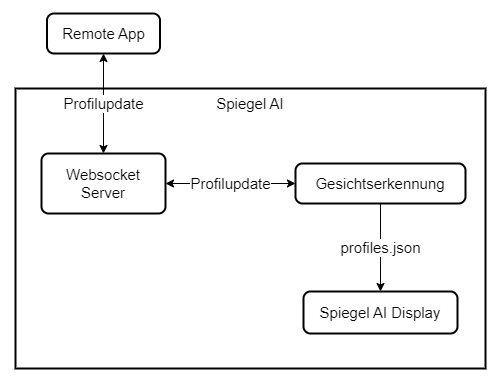
\includegraphics[width=0.7\textwidth]{pictures/websocket_diagram.png}
    \captionsetup{justification=centering, labelformat=simple, singlelinecheck=false}
    \caption{Darstellung der aktuellen Schnittstellen}
    \label{fig:websocket_diagram}
\end{figure} \\
Die finale Version der Schnittstellen wurde nach korrekter Profilverwaltung der Gesichtserkennung realisiert. Das Ziel war hier, die Websocket-Kommunikation zur Synchronisation der Profile zu nutzen, sodass das Display nicht mehr mit dem Server verbunden wird, sondern die Daten aus der lokalen \texttt{profiles.json}-Datei geladen werden. Um zu verstehen, wie eine Synchronisation erfolgreich implementiert werden kann, müssen einige Dinge berücksichtigt werden. Die Gesichtserkennung läuft dauerhaft und ist kontinuierlich mit dem Websocket verbunden. Die Remote App läuft auf einem Smartphone, welches die Verbindung beim Öffnen der App aufbaut, jedoch auch wieder trennt, wenn sie im Hintergrund läuft oder geschlossen wird. Das heißt, dass Änderungen des Profils am Spiegel AI stattfinden können, während die Remote App noch alte Profildaten enthält. Aus diesem Grund sendet die Spiegel AI Remote eine \texttt{fetch}-Nachricht an den Server, sobald eine Verbindung aufgebaut wird. Diese Nachricht wird von der Gesichtserkennung aufgenommen und löst das Senden der aktuellen Profile des Smart Mirrors aus. Somit läuft man nicht in Gefahr, dass die alten Profildaten im Smartphone die aktuellen Daten des Spiegels überschreiben. Eine weitere Änderung im Vergleich zur vorherigen Iteration war das Angeben eines \texttt{sender}. Dies stellt sicher, dass nur Nachrichten, welche nicht die eigens gesendet wurden, verarbeitet werden.

\section{Dynamische Widget Anordnung}
Erarbeitet von: Marcel Wagner \\ \\
Die Entwicklung eines Smart Mirrors mit dynamisch anpassbarer Display Anordnung stellt eine technische Herausforderung dar. Das Ziel dieses Bereiches war es, eine benutzerfreundliche und flexible Oberfläche zu schaffen, die sich den individuellen Präferenzen der Benutzer anpasst. Dieser Abschnitt beschreibt ausführlich die Methodik der Implementierung der dynamischen Display Anordnung sowie die dabei aufgetretenen Probleme und deren Lösungen. \\ \\
Ein essenzieller Bestandteil des Systems war die kontinuierliche Überwachung der 'profiles.json' Datei. Diese Datei wird von der Gesichtserkennung erstellt. Auf diesen Bereich wurde im vorherigen Kapitel bereits eingegangen. Hierzu wurde ein periodischer Abrufmechanismus implementiert, der alle 200 Millisekunden die Datei abfragt. Bei jeder Abfrage wurde der aktuelle Inhalt der Datei mit dem vorherigen Zustand verglichen, um Änderungen zu erkennen. Diese Methode stellte sicher, dass Anpassungen in den Benutzerprofilen zeitnah detektiert und umgesetzt wurden. \\ \\
Aus dieser Datei wird beginnend nach dem aktuellen ausgewählten Profil gesucht. Zur Identifikation des aktuell ausgewählten Profils wurde eine spezielle Funktion entwickelt. Diese Funktion durchsuchte die Liste der Profile nach dem als ausgewählt markierten Profil und gibt diese zurück. Ist kein Profil ausgewählt, wird null zurückgegeben, was die Anwendung des Standardzustands bedeutet. Die Fähigkeit, das aktive Profil zu identifizieren, war entscheidend für die Anpassung der Display Anordnung und stellte sicher, dass die Benutzereinstellungen korrekt umgesetzt wurden. \\ \\
Als nächster Schritt war ein weiterer zentraler Aspekt der Implementierung eine Funktion für die Ermittlung des aktuellen Zustands der Widgets. Hierbei wird das vorher ausgelesene Profil genutzt um hierfür den Zustand und Positionierung der Widgets auszulesen. Diese flexible Handhabung ermöglichte es, die Anzeige dynamisch an die individuellen Präferenzen der Benutzer anzupassen. \\ \\
Abschließend mussten noch auf Basis dieser Daten eine Dynamische Anpassung der HTML Seite vorgenommen werden.  Basierend auf dem aktuellen Zustand der Widgets wurden die entsprechenden HTML Elemente ein- oder ausgeblendet und in der gewünschten Reihenfolge angeordnet. Diese Anpassungen wurden durch die Funktion 'updateState' gesteuert, die die Widgets gemäß den Benutzereinstellungen neu positionierte. Die Funktion arbeitete folgendermaßen: Zunächst wird der Container, der die Widgets enthielt, geleert. Anschließend werden die Widgets gemäß der im Profil definierten Reihenfolge wieder hinzugefügt. Dabei wird auch die Sichtbarkeit jedes Widgets entsprechend dem enabled Status beachtet. Widgets, die nicht aktiviert waren, werden ausgeblendet, während aktivierte Widgets sichtbar blieben. Diese dynamische Anpassung ermöglichte es, die Widgets je nach Benutzerprofil in der gewünschten Anordnung und Sichtbarkeit darzustellen.

\subsection*{Aufgetretene Probleme und deren Lösung}
\textbf{Cache Verwaltung:} Das am häufigsten aufgetretene Problem war das der Cache Verwaltung des Browsers. Dies stellte eine besondere Herausforderung dar, da durch die regelmäßigen Anfragen an die 'profiles.json' Datei oft veralteter Inhalt aus dem Cache verwendet wurde, anstatt die neuesten Daten abzurufen. Dieses Problem wurde durch gezielte Deaktivierung des Caches für die betreffenden Anfragen gelöst. Der HTTP Header Cache Control wurde entsprechend konfiguriert, um sicherzustellen, dass die Anfragen stets frische Daten zurückliefert. Dies gewährleistete, dass immer die aktuellste Version der profiles.json Datei abgerufen und verarbeitet wurde, was eine zuverlässige Aktualisierung der Anzeige ermöglicht. \\ \\
\noindent
\textbf{CORS Beschränkung:} Ein weiteres Problem, welches während der Implementierung aufgetreten ist, war im Zusammenhang mit der Same Origin Policy des Browsers. Diese Sicherheitsrichtlinie verhinderte den Abruf der profiles.json Datei von einem anderen Ursprung, was die Aktualisierung der Profile erschwerte. Um dieses Problem zu umgehen, wurde ein lokaler Server mit Python erstellt, der die Datei ausliefert. Dieser Server ermöglichte es, die Datei lokal zu hosten und somit die CORS Beschränkungen (Cross Origin Resource Sharing) zu umgehen. Durch den Zugriff auf diesen lokalen Server konnte die Datei problemlos und sicher abgerufen werden, was die zuverlässige Aktualisierung der Profile gewährleistet.
\\ \\
\noindent
\textbf{Fehler bei der Skript ausführung:} Während der Implementierung der Dynamischen Widget Anordnung trat ein weitere Fehler auf, der verhinderte, dass das Skript in der 'updateState.js' Datei ausgeführt wurde. Um das Problem zu beheben war es für mich notwendig das Skript manuell in den code auszuführen. \\ \\
Durch diese manuelle Einbindung konnte der Fehler erfolgreich behoben und die korrekte Funktion des Skriptes sichergestellt werden. Diese Fehlerbehebung war notwendig um den weiteren Verlauf der Widget Anordnung zu gewährleisten.

